\chapter{Tutorial} %Soll der name verwendet werden? [janp]
%Wenn name geändert wirt, referenzen auf name Prüfen!

\section{Einrichten eines neuen Microcotrollers}
Für unser Projekt sollen alle notwendigen Programmbestandteile sowie die gesamte
Website auf dem Microcotnroller gespeichert werden. Der beim AVR-Net-IO
mitgelieferte ATmega32 bietet hierfür jedoch nicht ausreichend Speicher.
Wir haben uns deswegen für den aus der gleichen Baureihe stammenden ATmega644P
entschieden der mit seinen 64KB Programmspeicher den doppelten Speicherplatz
bietet als der kleinere ATmeag32.

Für einen neuen Chip ist es anfangs notwendig die Fuse-Bits richtig zu setzen,
damit der Chip Ordnungsgemäß Arbeitet.
Dies ist jedoch im AtmelStudio nicht Möglich, da es nicht möglich ist die exakte
Geräte-Signatur auszulesen.
Das Problem liegt darin, das Standartmäßig die Fuses auf den internen
Quarz-Kristall gesetzt sind und nicht auf den Externen Kristall des
AVR-NET-IO Boards.
Beim versuch die Fuse-Bits zu setzen wird man im Atmel Studio mit folgender
Fehlermeldung begrüßt. 
\begin{figure}[h]
\centering
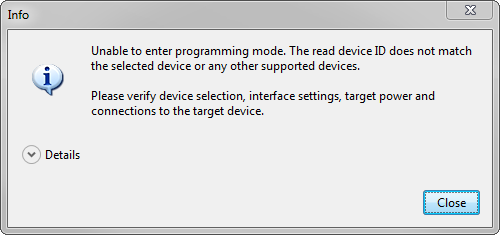
\includegraphics[width=13cm]{content/pictures/Anleitung/neuerProzessor/AnleitungNeuerProzessor2_fehler.png}
\caption{DeviceProgramming}
\end{figure}

Abhilfe Schafft hier die Alternative Programmiersoftware AVRDUDE, mit ihr ist
es Möglich die Fuse-Bits zu ändern. Unter Linux kann dieser einfach über die
Paketquellen installiert werden, für ein Windows Betriebssystem kann eine
ausführbare Kommandozeilen-Anwendung auf der Projekt-Website heruntergeladen
werden \url{http://savannah.nongnu.org/projects/avrdude}. Zusätzlich muss für
windows noch libusb-win32 (\url{http://sourceforge.net/projects/libusb-win32/})
vorhanden sein, das der Programmer mit den gewählten Parametern verwendet werden
kann. Eine ausfühliche anleitung gibt es hier:
\url{http://eliaselectronics.com/using-the-avrispmkii-with-avrdude-on-windows/}


\begin{table}[H]
\begin{tabular}{| p{.24\textwidth} | p{.76\textwidth} |}
\hline
Auslesen Linux:& sudo avrdude -P usb -p m644p -c avrispmkII  -U lfuse:r:-:h -U hfuse:r:-:h -B 22 \\ \hline
Setzen Linux:& sudo avrdude -P usb -p m644p -c avrispmkII -U lfuse:w:0xFF:m -U hfuse:w:0xD6:m -B 22 \\ \hline
Auslesen Windows:& avrdude.exe -p m644p -c avrispmkII -U lfuse:r:-:h -U hfuse:r:-:h -B 22 \\ \hline 
Setzen Windows:& avrdude.exe -p m644p -c avrispmkII -U lfuse:w:0xFF:m -U hfuse:w:0xD6:m -B 22 \\ \hline
\end{tabular}
\caption{Auslesen und setzen von Fuse-Bits mit dem AVRDUDE}
\label{tablelabel}
\end{table}
Die Ausgabe von AVRDUDE beim setzen der neuen Fuse-Bit Einstellungen.

\begin{figure}[h]
\centering
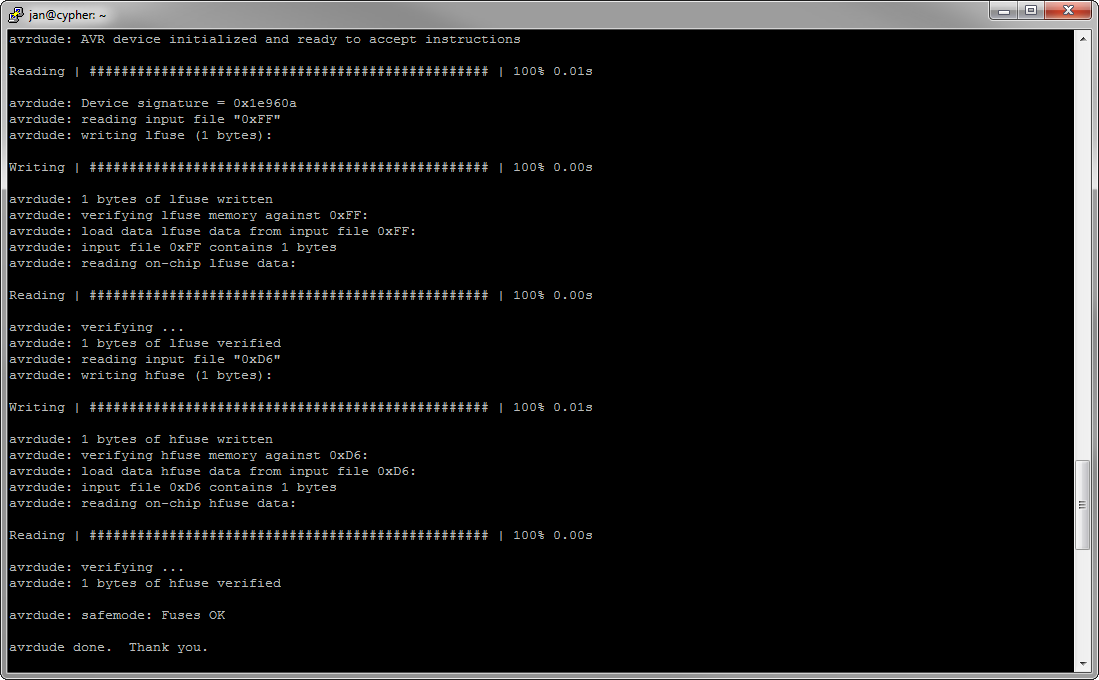
\includegraphics[width=13cm]{content/pictures/Anleitung/neuerProzessor/avrOutput.png}
\caption{AVRDUDE Ausgabe}
\end{figure}

Ein Auszug der verwendeten Parameter aus der AVRDUDE Handbuch Seite:

\begin{table}[H]
\begin{tabular}{| p{.35\textwidth} | p{.65\textwidth} |}
\hline
-p partno & This is the only option that is mandatory for every invocation of
avrdude.  It specifies the type of the MCU connected to the programmer. These
are read from the config file.  If avrdude does not know about a part that you
have, simply add it to the config file (be sure and submit a patch back to the
author so that it can be incorporated for the next version). \newline
\textbf{m32 $\Rightarrow$ ATmega32} \newline 
\textbf{m644p $\Rightarrow$ ATmega644P} \newline
\textbf{m1284p $\Rightarrow$ ATmega1284P} \\ \hline
-P port & Use port to identify the device to which the programmer is attached. \textbf{usb für den AVRISP MKII}  \\ \hline 
-c programmer-id & \textbf{avrispmkII für den AVRISP MKII} \\ \hline
-U \hbox{memtype:op:filename:filefmt} &  
The \textrm{memtype} field specifies the memory type to operate on.\newline
\textbf{hfuse} The high fuse byte.\newline
\textbf{lfuse} The low fuse byte.\newline
The \textrm{op} field specifies what operation to perform:\newline
\textbf{r} read device memory and write to the specified file\newline
\textbf{w} read data from the specified file and write to the device memory \newline
The filename field indicates the name of the file to read or write.  The format field is optional and contains the format of the file to read or write. \newline
\textbf{Hier die Bytes die gesetzt werden 0xFF bzw 0xD6}
\\ \hline
-B bitclock & Specify the bit clock period for the JTAG interface or the ISP clock \\ \hline
\end{tabular}
\caption{Auslesen und setzen von Fuse-Bits mit dem AVRDUDE}
\label{tablelabel}
\end{table}

Anschließend kann der Mikrocontroller zusammen mit dem AV-Net-IO und AtmelStudio
Programmiert werden. Der Verwendete Mikrocontroller wird jetzt richtig erkannt,
da es auch keine Probleme mit der Gerätesignatur gibt.

\section{HTML Header Compiler}

Parameter und Funktionsweise

\section{Hexfiles Überspielen}

Zum übertragen der Hexfiles gibt es verschiedene Möglichkeiten.

\subsection{AVRDUDE}



\subsection{Atmel Studio}

\section{Die Website}
